\chapter*{Introduction to photoacoustics}
\addcontentsline{toc}{chapter}{Introduction to photoacoustics}

In order to detect the absorption lines of \ce{O2} in the visible region, we did a photoacoustic measurement. This kind of measurement turns useful every time one is interested in the absorption properties of a gas, but the absorption is too weak to be detected via a standard measurement. This can happen because the pressure of the studied gas is very low, or because it is very diluted into a mix of other gases, or just because the gas has a very poor response to a certain frequency stimulation, which is the case of the oxygen at visible frequencies. A standard measurement of absorbance is basically just a difference between the intensity of the impinging light and that of the light passed through the gas, so that one can account for the photons which were absorbed by looking how much light fails to exit the champion.

\begin{wrapfigure}{r}{6.5cm}\centering
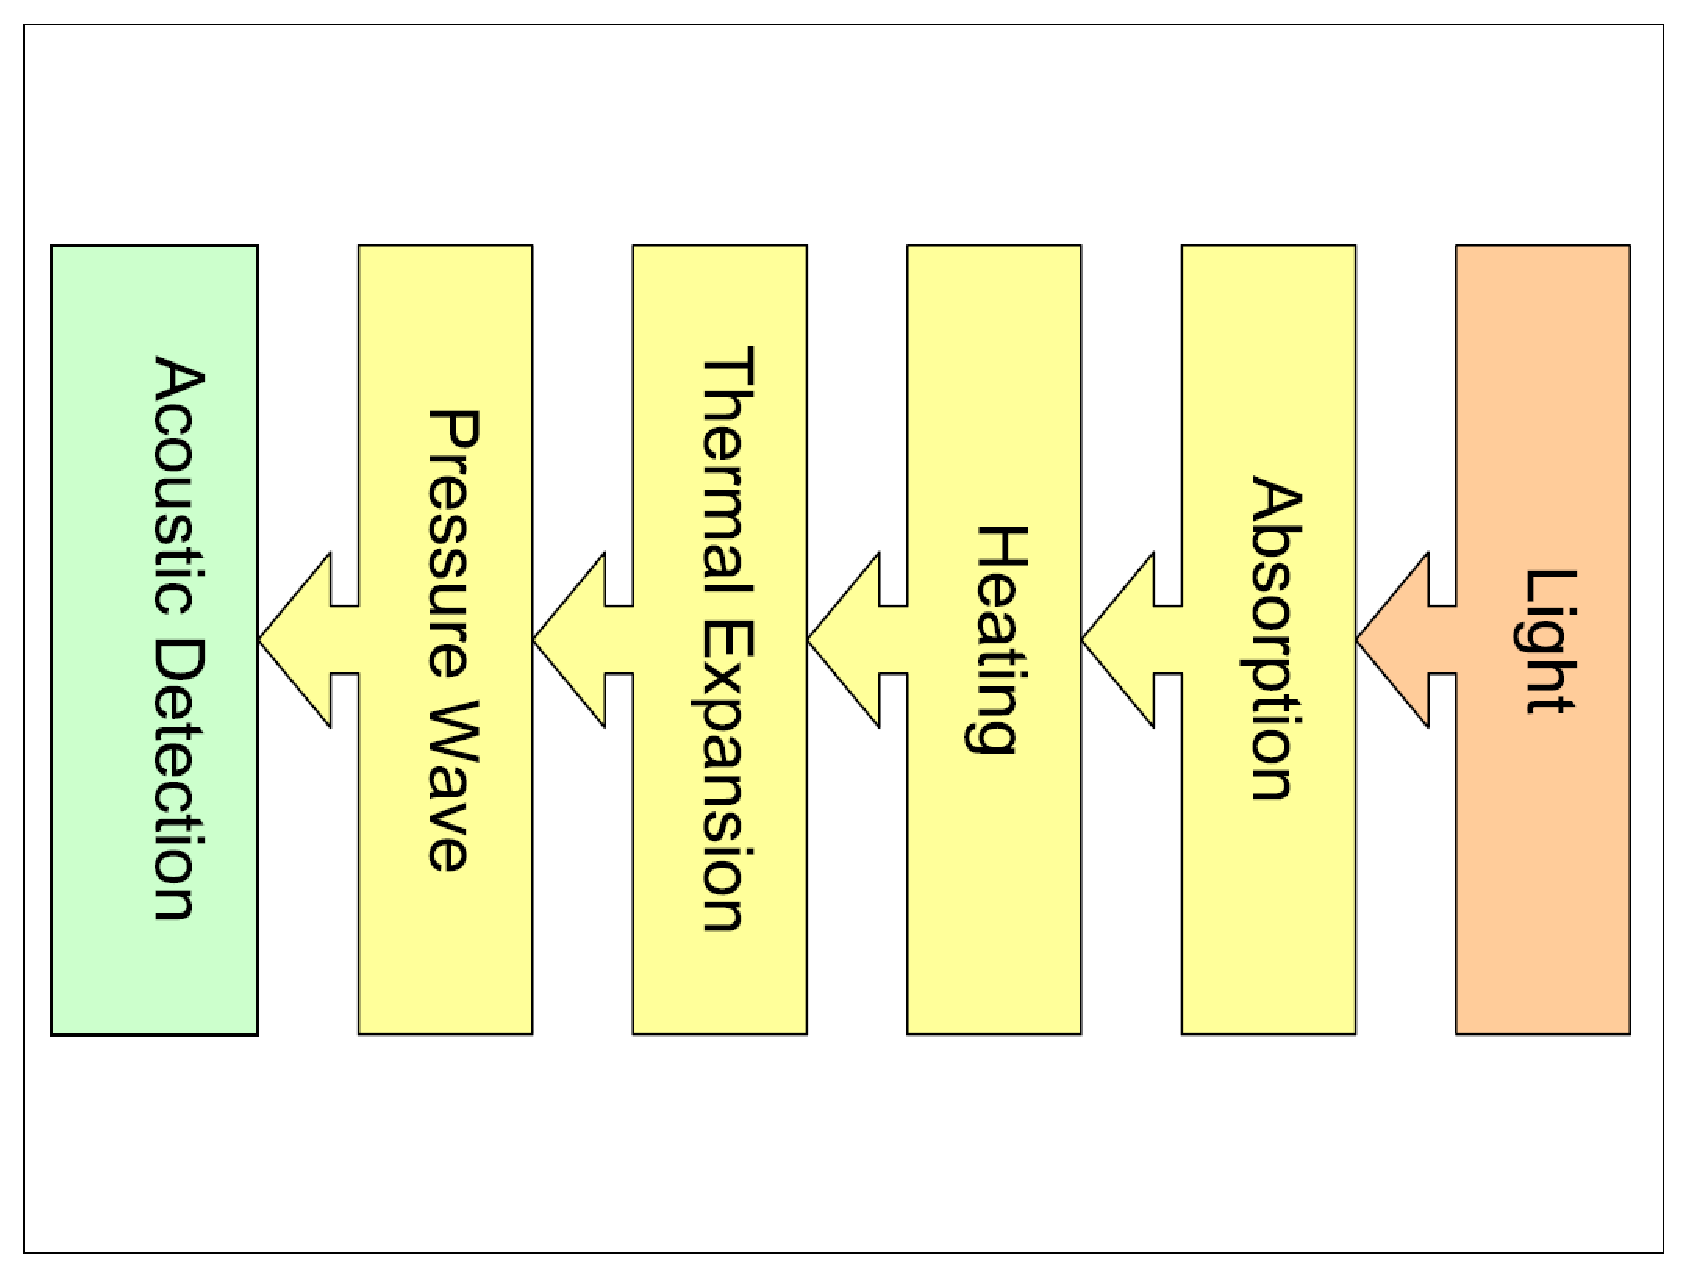
\includegraphics[width=\linewidth, angle=90, draft=false]{eps/photoacoustics.eps}
\caption{Steps of a photoacoustic measurement.}
\label{photoacoustics}
\end{wrapfigure}
Photoacoustics exploits a different mechanism (\cref{photoacoustics}), as it considers directly the effect the absorbed light has on the gas. In fact, the photons absorbed by the gas molecules excite electronic or vibronic modes (depending on the frequency). Apart for the case of fluorescence or phosphorescence (phenomena which usually happen exciting atomic modes and not molecular ones), the excited molecules subsequently relax, releasing their energy in form of heat. This leads to a pressure increase in the gas. If the exciting light is modulated in frequency, which is the case for a laser passing through a chopper, one gets the pressure to increase and decrease at the chopping frequency, which means a sound wave is generated that can be detected by a microphone. 
To enhance the signal, the chopping usually happens at the first longitudinal resonant frequency of the chamber, so that the maximum acoustic signal is found in the center. Incidentally, the chopper modulation allows also the exploitation of a lock-in amplifier, which further improves the sensibility of this configuration to small absorption signals.